\section{Introduction}

\setlength{\tabcolsep}{2pt}
\begin{figure}
\begin{center}
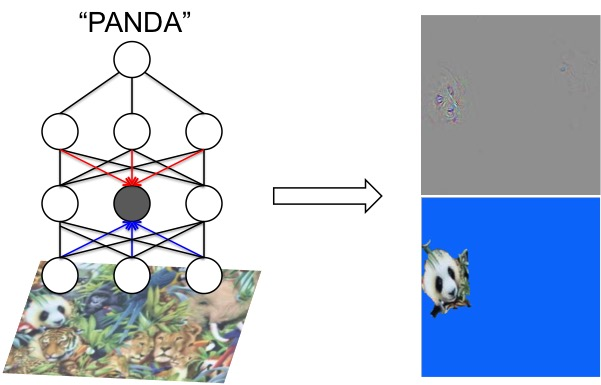
\includegraphics[width=0.95\columnwidth]{figs/splash0/splash0}
% \vspace{-10pt}
\caption{We propose a novel feedback convnet for weakly supervised object localization in complex scenes with cluttered background. The feedback net is able to utilized both bottom-up image features and top-down semantic labels to infer the hidden layer neuron status to match the localize the correponding salient area in the image. }
\label{fig:splash0}
% \vspace{-30pt}
\end{center}
\end{figure}

\setlength{\tabcolsep}{2pt}
\begin{figure*}
\begin{center}
\begin{tabular}{ccccccc}
%\rotatebox{90}{\hspace{5mm}Sequential} &
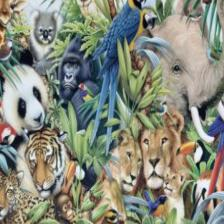
\includegraphics[width=0.13\linewidth]{figs/splash/original} &
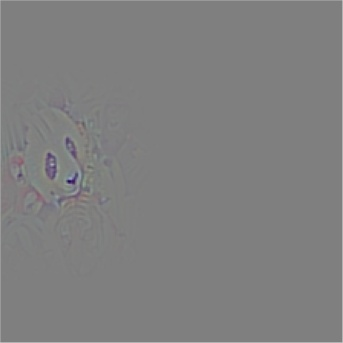
\includegraphics[width=0.13\linewidth]{figs/splash/panda} &
\includegraphics[width=0.13\linewidth]{figs/splash/tiger} &
\includegraphics[width=0.13\linewidth]{figs/splash/gorilla} &
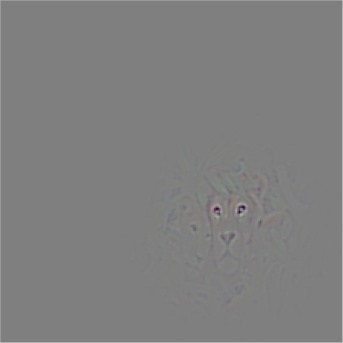
\includegraphics[width=0.13\linewidth]{figs/splash/lion} &
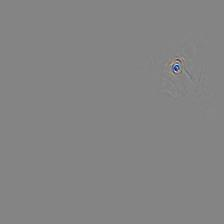
\includegraphics[width=0.13\linewidth]{figs/splash/elephant} &
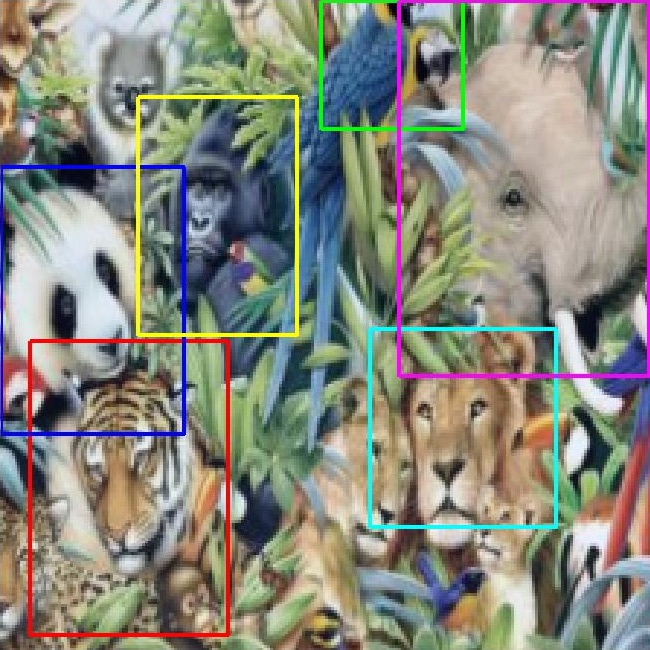
\includegraphics[width=0.13\linewidth]{figs/splash/localization}\\
{\small (a) Input Image} &
{\small (b) Panda} &
{\small (c) Tiger} &
{\small (d) Gorilla} &
{\small (e) Lion} &
{\small (f) Elephant} &
{\small (g) Localization}
\end{tabular}
% \vspace{-10pt}
\caption{We illustrate the localization power of the feedback net on a multi-object image with cluttered background. (a) shows the original input image which both VggNet and GoogleNet recongize as "comic". (b) - (f) demonstrate the powerfulness of our model understanding the image given paticular object labels. We visualization the gradient of each label w.r.t. image after ther convergence of the feedback neural nets (g) shows the localization power for different objects in this complex image based on the gradient. Note that the weights in the net is obtained from a pre-trained feedforward GoogleNet model for image classification.}
\label{fig:splah}
% \vspace{-30pt}
\end{center}
\end{figure*}

\setlength{\tabcolsep}{2pt}
\begin{figure*}
\begin{center}
\begin{tabular}{ccccccccc}
\rotatebox{90}{\hspace{5mm}Oxford} &
\includegraphics[width=0.11\linewidth]{figs/visual_compare/gradient/oxford/panda} &
\includegraphics[width=0.11\linewidth]{figs/visual_compare/saliency/oxford/panda} &
\includegraphics[width=0.11\linewidth]{figs/visual_compare/gradient/oxford/tiger} &
\includegraphics[width=0.11\linewidth]{figs/visual_compare/saliency/oxford/tiger} &
\includegraphics[width=0.11\linewidth]{figs/visual_compare/gradient/oxford/gorilla} &
\includegraphics[width=0.11\linewidth]{figs/visual_compare/saliency/oxford/gorilla} &
\includegraphics[width=0.11\linewidth]{figs/visual_compare/gradient/oxford/lion} &
\includegraphics[width=0.11\linewidth]{figs/visual_compare/saliency/oxford/lion} \\
\rotatebox{90}{\hspace{5mm}Deconv} &
\includegraphics[width=0.11\linewidth]{figs/visual_compare/gradient/deconv/panda} &
\includegraphics[width=0.11\linewidth]{figs/visual_compare/saliency/deconv/panda} &
\includegraphics[width=0.11\linewidth]{figs/visual_compare/gradient/deconv/tiger} &
\includegraphics[width=0.11\linewidth]{figs/visual_compare/saliency/deconv/tiger} &
\includegraphics[width=0.11\linewidth]{figs/visual_compare/gradient/deconv/gorilla} &
\includegraphics[width=0.11\linewidth]{figs/visual_compare/saliency/deconv/gorilla} &
\includegraphics[width=0.11\linewidth]{figs/visual_compare/gradient/deconv/lion} &
\includegraphics[width=0.11\linewidth]{figs/visual_compare/saliency/deconv/lion} \\
\rotatebox{90}{\hspace{5mm}Our} &
\includegraphics[width=0.11\linewidth]{figs/visual_compare/gradient/feedback/panda} &
\includegraphics[width=0.11\linewidth]{figs/visual_compare/saliency/feedback/panda} &
\includegraphics[width=0.11\linewidth]{figs/visual_compare/gradient/feedback/tiger} &
\includegraphics[width=0.11\linewidth]{figs/visual_compare/saliency/feedback/tiger} &
\includegraphics[width=0.11\linewidth]{figs/visual_compare/gradient/feedback/gorilla} &
\includegraphics[width=0.11\linewidth]{figs/visual_compare/saliency/feedback/gorilla} &
\includegraphics[width=0.11\linewidth]{figs/visual_compare/gradient/feedback/lion} &
\includegraphics[width=0.11\linewidth]{figs/visual_compare/saliency/feedback/lion} \\
&
\multicolumn{2}{c}{{\small (a) Panda}} &
\multicolumn{2}{c}{{\small (b) Tiger}} &
\multicolumn{2}{c}{{\small (c) Gorilla}} &
\multicolumn{2}{c}{{\small (d) Lion}} \\
\end{tabular}
% \vspace{-10pt}
\caption{We demonstrate the effectiveness of our method by comparing the class model visualization results against Oxford [] and Deconv []. The input image is the same as Figure 1 (a). We show both the visualization results as well as the saliency map. While both Oxford and Deconv have the same input: the image and an object class label (i.e. tiger, panda, etc.), the gradients computed are often salient on one particular object (i.e. elephant). Our feedback framework allows for the model to focus on the most important image area that improves the class confidence.}
\label{fig:visual_compare}
% \vspace{-30pt}
\end{center}
\end{figure*}


~\cite{a}
We present a novel feedback neural networks for joint reasoning the class node and hidden layer information. The network is powerful to be applied on model class visualization and object localization even in cluttered scenes with multi objects. The framework is novel and 

\textbf{Deep Learning and Deep Convolutional Neural Networks, Feedforward Strcture}

\textbf{Psychological feedback, inference top-down and bottom-up}

\textbf{This paper Main Contribution}

\textbf{Yurgen's feedback neural networks, Attention neural networks, Deep Boltzman Machines}

\textbf{Comparing against Oxford and Deconv}

\textbf{ConvNet Implementation Details}
